\subsection{Расчет скоростей нейтронного захвата с помощью TALYS}
Скорость ядерной реакции $\lambda$ рассчитывается путем свертки ее сечения с энергетическим распределением взаимодействующих частиц. Энергии нейтронов и ядер в звездном веществе имеют распределение Максвелла-Больцмана. Следует учитывать, что при астрофизических температурах ядра находятся в возбужденных состояниях, и в условиях термодинамического равновесия заселенность уровней также должна подчиняться статистике Максвелла-Больцмана. Тем самым формула для астрофизической скорости ядерной реакции, являющейся функцией температуры среды $T$, принимает вид
\begin{equation}
\displaystyle
\lambda(T) = \sqrt{\frac{8}{\pi m}} \frac{N_A}{(k T)^{3/2} G(T)} \int_0^\infty \sum_\mu \frac{(2 I^\mu + 1)}{(2 I^0 + 1)} \sigma^\mu(E) E \exp \left( - \frac{E + E_x^\mu}{kT} \right) dE,
\end{equation}
где $E^\mu_x$ и $I^\mu$ --- энергия и спин возбужденного уровня $\mu$, $m$ --- приведенная масса взаимодействующих частиц, $k$ --- постоянная Больцмана, $N_A$ --- число Авогадро, $G(T)$ --- статистическая сумма
\begin{equation}
    \displaystyle
    G(T) = \sum_\mu \frac{(2 I^\mu + 1)}{(2 I^0 + 1)} \exp \left( - \frac{E_x^\mu}{kT} \right)
\end{equation}

Расчет скорости ядерной реакции требует предварительного расчета зависимости ее сечения от энергии взаимодействия $\sigma(E)$. В настоящей работе рассматривается эволюция астрофизической ядерной системы при температурах не более $6$~ГК. Энергии нейтронов при таких условиях достаточно малы, чтобы реакцию $(n,\gamma)$ можно было рассматривать с точки зрения статистической модели. В настоящей работе скорости астрофизических скоростей реакций нейтронного захвата рассчитывались при помощи программы TALYS с использованием различных моделей ядерных масс. 

Программа TALYS позволяет производить расчеты сечений и астрофизических скоростей ядерных реакций с возможностью задания различных параметров статистической модели, например, теоретических значений масс ядер. По умолчанию программа использует таблицы масс ядер, рассчитанные при помощи обсужденных моделей FRDM2012~\cite{moller2016}, HFB-24~\cite{goriely2013}, а также HFB D1M~\cite{goriely2009}, которая является вариантом метода Хартри-Фока-Боголюбова с потенциалом Гоньи. Чтобы использовать другие массовые модели, их результаты нужно перевести в формат таблиц, используемый TALYS, подробно описанный в руководстве к программе. В TALYS также внесена таблица экспериментальных масс, построенная на основе базы данных AME2003~\cite{wapstra2003}, их использование включается отдельным параметром при запуске расчета. Наконец, если при расчете TALYS требуются значения масс, отсутствующие в заданной теоретической таблице, то программа использует аналитическую формулу Дуфло-Цукера~\cite{duflo1995}.

В настоящей работе для расчета астрофизических скоростей реакции нейтронного захвата использовались микро-коллективная модель FRDM2012, микроскопическая модель HFB-24, а также феноменологический метод LMR2021, результаты которого были переведены нами в формат TALYS. В настоящей работе не приведены результаты расчетов с массовой моделью HFB D1M, так как она отличается от HFB-24 в основном лишь выбором потенциала.

\begin{figure}
  \centering
  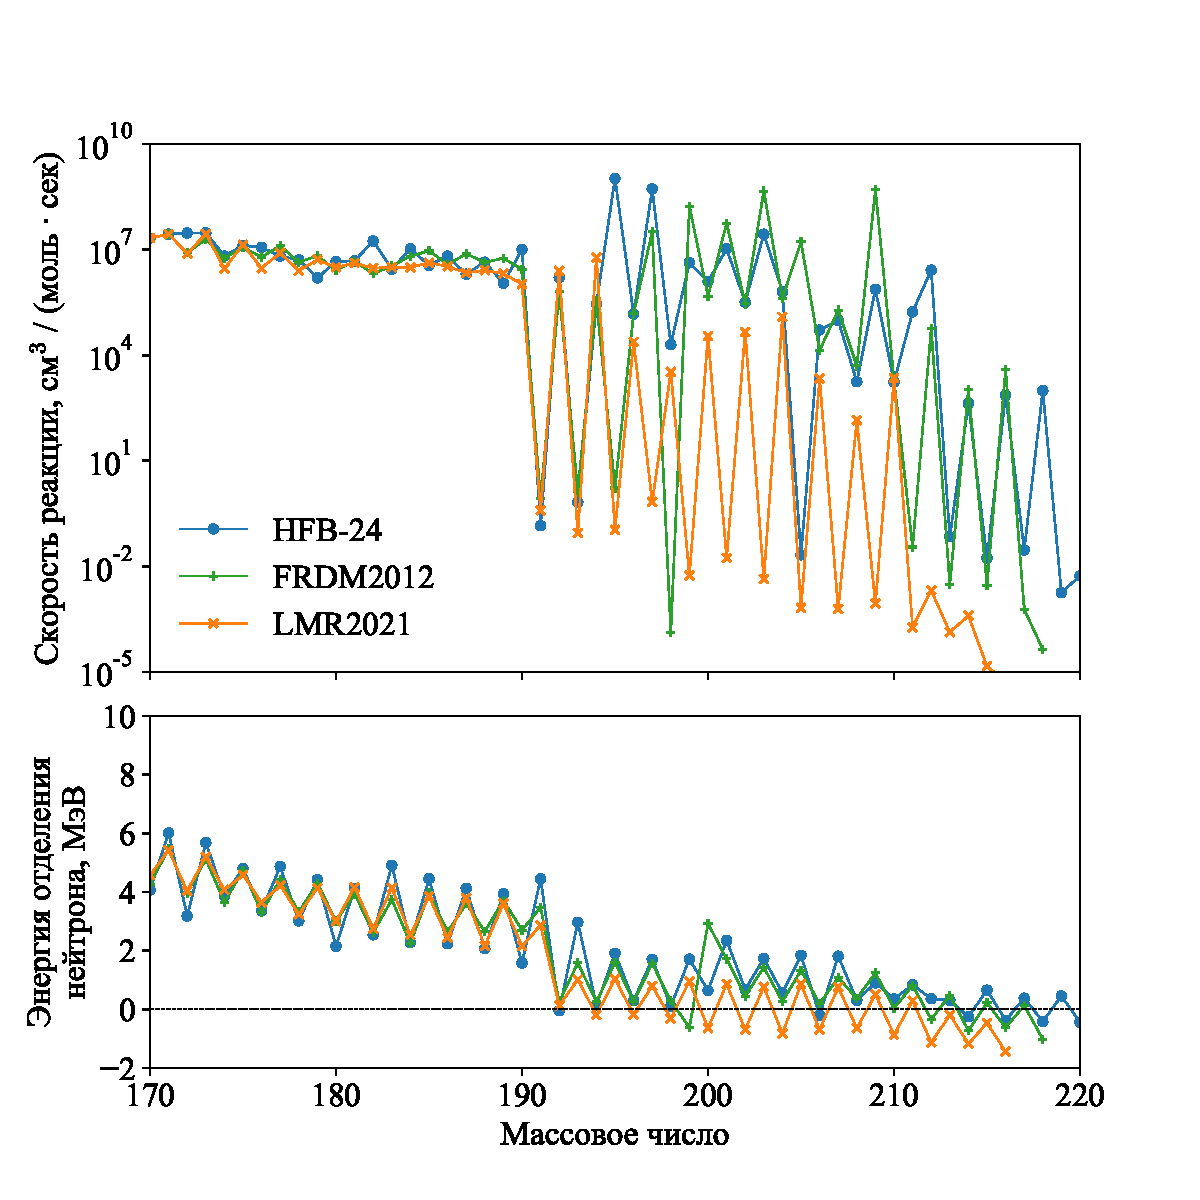
\includegraphics[width=0.6\textwidth]{pics/rates_vs_A_tb.pdf}
  \caption{Свреху: скорости нейтронных захватов на нейтроноизбыточных изотопах тербия, рассчитанные с помощью различных таблиц ядерных масс. Снизу: энергии отделения нейтронов для нейтроноизбыточных изотопов тербия по данным тех же массовых таблиц.}
  \label{fig:rates_vs_A}
\end{figure}

